\section{Methods}
\label{sec:methods}

\subsection{Related work}

There are already existing APIs or tools to download, inference and train AI
models:
\begin{itemize}
  \item Transformers (Hugging Face API) \cite{wolf-etal-2020-transformers}
  \item Cellpose API \cite{Stringer2020.02.02.931238}
  \item BioImage.IO Core (Python libraries)
  \item SAM2 repository \cite{ravi2024sam2}
\end{itemize}

\subsection{No common APIs}

The problem is there are no common APIs/\Gls{CLI}s/no standard.

For example with 'download API', there are four differents code for these four
repositories:
\begin{itemize}

  \item BioImage.IO code
  \begin{minted}[frame=lines,framesep=2mm,baselinestretch=0.8,fontsize=\small,linenos]{python}
  model = load_description(args.model)
  \end{minted}

  \item Hugging Face code
  \begin{minted}[frame=lines,framesep=2mm,baselinestretch=0.8,fontsize=\small,linenos]{python}
  pipe = pipeline(task="mask-generation",
                  model=args.model,
                  points_per_batch=32,
                  device=device)
  \end{minted}

  \item SAM2 code
  \begin{minted}[frame=lines,framesep=2mm,baselinestretch=0.8,fontsize=\small,linenos]{python}
  mask_generator = SAM2AutomaticMaskGenerator
    .from_pretrained(args.model,
                     device=device)
  \end{minted}

  \item Cellpose code
  \begin{minted}[frame=lines,framesep=2mm,baselinestretch=0.8,fontsize=\small,linenos]{shell-session}
  $ python -m cellpose\
      --pretrained_model cyto3\
      --dir {inputs}\
      --savedir {output}
  \end{minted}
\end{itemize}

There is the same issue with 'inference API', 'train API', etc.

\subsection{Our approach}

We use existing APIs of AI repositories and use them in the context of
\Gls{WIPP}. We use \Gls{AiModelCard} to document AI model trained in WIPP.

Our contributions are:
\begin{itemize}
  \item Analyze API of AI repositories
  \item Implement them for containerized plugin that run in WIPP without learning the API
  \item Trained/retrained AI model will comes with proper AI model card
\end{itemize}

\subsection{Web Image Processing Pipelines}

WIPP is a scientific workflow engine, illustrated as shown in figure 1.
The purpose of this tool is to make measurements based on terabyte-sized images.
It is an algorithmic plugin platform. Its goal is to lower the bar to execute
image analyses.

\begin{figure}[H]
  \centering
  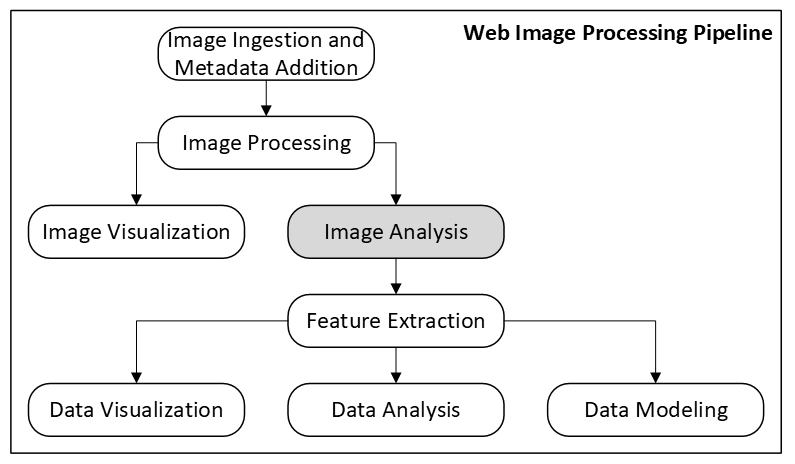
\includegraphics[width=1.0\linewidth]{png/methods/wipp.png}
  \caption{WIPP}
  \label{fig:1wipp}
\end{figure}

WIPP worflows are sequence of plugins. WIPP plugins are piece of code (code put
in the form of a container) taking inputs and outputs and executing code.

Thanks to a plugin you can, for example, load an AI model hosted in
WIPP, specify an
image collection and perform the AI inference of this AI model on the
selected images.
The result will be a new collection of images modified by the AI model, for
example
with a label after inference of a \Gls{ClassificationModel}.

\subsection{Access public AI repositories}

There are many public AI models on lots of public AI repositories.

\begin{table}[H]
  \centering
  \caption{Number of models per repository}
  \begin{tabular}{lcc}
    \toprule
    AI repositories & IC models & S + MG models \\
    \midrule
    Hugging Face    & 15,593                      & 1,160 + 176 \\
    BioImage.IO     & 1                           & 4 + 32 \\
    Cellpose        & $\times$                    & 21 \\
    SAM2            & $\times$                    & 8 \\
    PyTorch Hub     & 20                          & 5 \\
    \bottomrule
  \end{tabular}
  \caption*{Image Classif. (IC), Segmentation (S), Mask Generation (MG)}
\end{table}

Our goal is to access external AI models in WIPP.


We have developed new inference plugins, see figure 2, to enable access to
AI models available on different public AI repositories such as
Hugging Face, BioImage.IO, Cellpose, and more.

\begin{figure}[H]
  \centering
  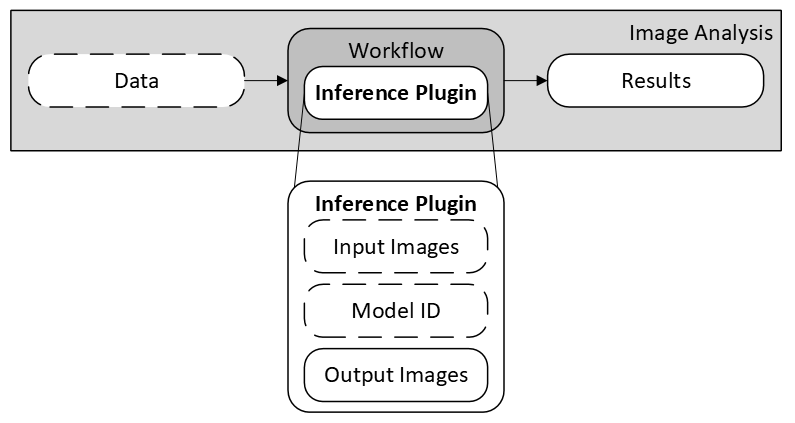
\includegraphics[width=1.0\linewidth]{png/methods/inference_plugin.png}
  \caption{Inference Plugin}
  \label{fig:2inference}
\end{figure}

This was achieved by developing general-purpose code using the API of
the various platforms. This
enabled us to increase the number of AI models usable
in WIPP thanks to containerized software.

\subsection{Document AI models}

We have introduced AI model card entries that are necessary for matching tasks
with AI models. This information will also be needed as runtime parameters.
Figure 3, training an AI in WIPP automatically generates its documentation
(AI model card).

\begin{figure}[H]
  \centering
  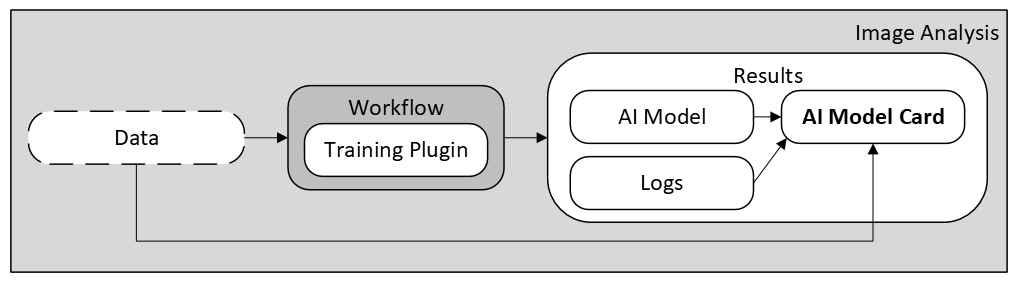
\includegraphics[width=1.0\linewidth]{png/methods/ai_model_card.png}
  \caption{AI model card}
  \label{fig:3aimodelcard}
\end{figure}

This was achieved by developing code to retrieve information about the AI model
throughout the pipeline: name, creation date, data used for training, number of
iterations, training time, and more.

\subsection{Compute accuracy}

Our goal is to mesure accuracy of external AI results and to select the most
accurate/fastest one.

We have developed a new plugin, see figure 4, to compute the \Gls{DiceIndex}.

The formula is:

\[ Dice = \frac{2*TP}{2*TP + FP + FN} \]

It is a statistic used to gauge the similarity of two samples, in
our case images.

\begin{figure}[H]
  \centering
  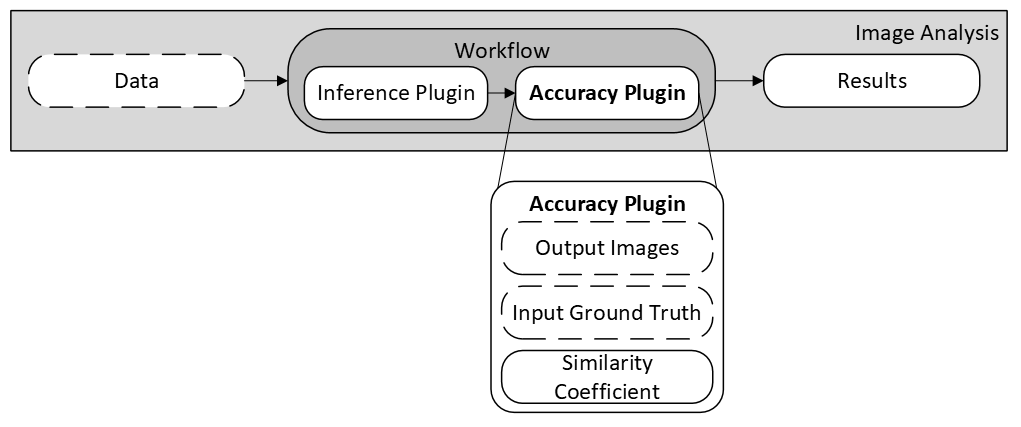
\includegraphics[width=1.0\linewidth]{png/methods/accuracy.png}
  \caption{Accuracy Plugin}
  \label{fig:4accuracy}
\end{figure}

This was achieved by implementing the Dice index's formula into a containerized
software (plugin). This makes it now possible to sequence model AI inference (a
model created within WIPP or a model from a repository) and evaluate the
accuracy of the result provided, by comparing it with
\Gls{GroundTruthData}.
